
\subsection{Torque--speed envelope and efficiency}
\Cref{fig:tn} shows the motor torque--speed envelope at a \SI{48}{V} bus with an efficiency map underneath. The envelope comes from a $dq$ model whose $q$-axis torque follows the 3-D sweep of \cref{tab:sweep}, i.e.\ $\psi_\mathrm{eff}(I)=T(I)/(\tfrac32pI)$. It uses $\psi_m=\SI{8.62}{mWb}$, $L_d=L_q=\SI{52}{\micro H}$, $R=\SI{37.5}{m\ohm}$ (\SI{100}{\celsius}), modulation index 0.96, $|i_d|\le\SI{120}{A}$, and the minimum-current $(i_d,i_q)$ pair at every operating point. The losses are copper loss with a Dowell AC factor $1+0.3(f/\SI{550}{Hz})^2$, core loss scaled from the motor-thread Steinmetz estimate, \SI{10}{W} of rotor eddy loss at \SI{2200}{rpm} scaling with $n^2$, and an assumed \SI{0.02}{\Nm} bearing drag. The map is motor-only: inverter and gearbox losses are excluded.
The constant-torque region extends to about \SI{90}{rad/s} (\SI{14}{rad/s} at the output), after which field weakening holds useful torque to the edge of the plot. Peak efficiency is 94\,\% at moderate torque and \SIrange{150}{220}{rad/s}. In the high-torque, low-speed region used in stance, efficiency is low (below 50\,\%) because copper loss dominates. This is the reason the thermal limit, not the envelope, governs locomotion.

\begin{figure}[!t]
\centering
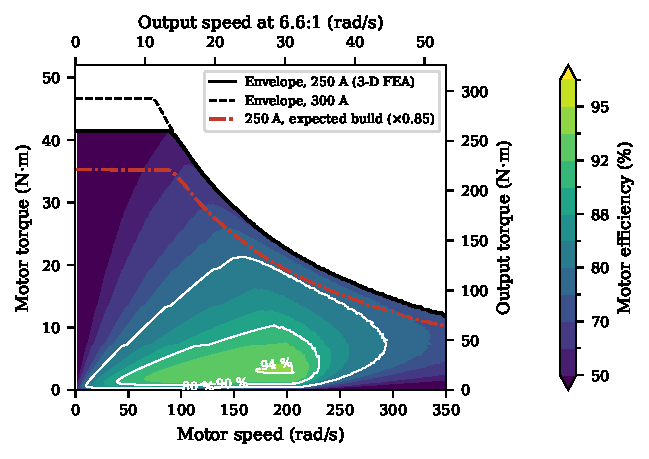
\includegraphics[width=\columnwidth]{tn_eff.pdf}
\caption{Motor torque--speed envelope at \SI{48}{V} (\SI{250}{A}, solid; \SI{300}{A}, dashed; expected built motor at 0.85$\times$, dash-dot) over the motor efficiency map, with output-shaft axes for the 6.6:1 reduction ($\eta=0.95$).}
\label{fig:tn}
\end{figure}

\subsection{Thermal endurance: constant versus sinusoidal current}
The winding-temperature limit is evaluated with the four-node lumped model of the motor design thread: winding, core, housing and ambient. The stator is v0.4.10 ($R_{20}=\SI{28.5}{m\ohm}$, winding capacity about \SI{88}{J/K}), the housing-to-air resistance is \SI{1}{K/W}, and each run starts at \SI{40}{\celsius}. Two duty types are compared in \cref{fig:thermal,tab:thermal}:
\begin{itemize}
\item \emph{constant peak}: the current amplitude is held at $I$, as in a static hold or a sustained push, so copper loss is $\tfrac32I^2R$;
\item \emph{sinusoidal}: the torque command swings sinusoidally between $+I$ and $-I$ with a \SI{0.4}{s} stride period, as in a locomotion gait. Mean copper loss is then half as large.
\end{itemize}
The sinusoidal case is the more relevant one for running. It reaches \SI{150}{\celsius} after about \SI{8}{s} at \SI{250}{A} and \SI{16}{s} at \SI{200}{A}, compared with \SI{3.4}{s} and \SI{5.9}{s} at constant current. The ratio grows from about 2.4 at high current to 3 or more at low current, because the winding and core thermal capacitances absorb the oscillating part of the loss.

\begin{figure}[!t]
\centering
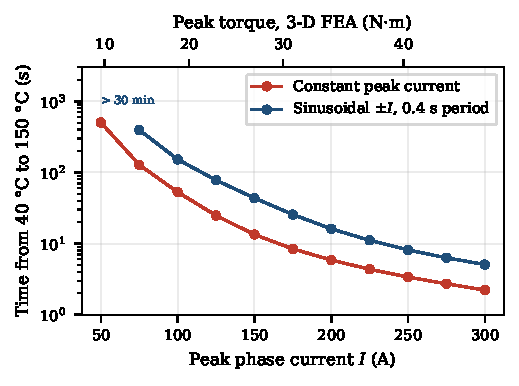
\includegraphics[width=\columnwidth]{thermal_t150.pdf}
\caption{Time for the winding to rise from \SI{40}{\celsius} to \SI{150}{\celsius} against peak current, for constant current and for a sinusoidal $\pm I$ trajectory with \SI{0.4}{s} period. Top axis: corresponding peak torque from the 3-D model.}
\label{fig:thermal}
\end{figure}

\begin{table}[!t]
\caption{Time from \SI{40}{\celsius} to \SI{150}{\celsius} winding temperature (s)}\label{tab:thermal}
\centering\footnotesize
\begin{tabular}{@{}rrrr@{}}
\toprule
$I$ (A, peak) & Constant & Sinusoidal $\pm I$ & Ratio\\
\midrule
50 & 502 & $>$1800 & --\\
75 & 128 & 395 & 3.1\\
100 & 52.9 & 152 & 2.9\\
125 & 24.8 & 77.7 & 3.1\\
150 & 13.4 & 43.5 & 3.3\\
175 & 8.4 & 25.6 & 3.0\\
200 & 5.9 & 16.1 & 2.8\\
225 & 4.4 & 11.1 & 2.5\\
250 & 3.4 & 8.1 & 2.4\\
275 & 2.7 & 6.3 & 2.3\\
300 & 2.2 & 5.1 & 2.3\\
\bottomrule
\end{tabular}
\end{table}
